\setAuthor{Mihkel Kree}
\setRound{lahtine}
\setYear{2015}
\setNumber{G 7}
\setDifficulty{7}
\setTopic{Vedelike mehaanika}

\prob{Veejoad}
\begin{wrapfigure}{r}{0.2\textwidth}%
\vspace{-15pt}
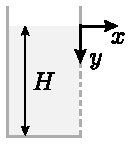
\includegraphics[width=\linewidth]{2015-lahg-07-veejoadJoon}%
\end{wrapfigure}
Vertikaalse silindrilise anuma seina sisse on paljudele erinevatele kõrgustele tehtud pisikesed augud, millest voolab välja vett. Anumasse valatakse aeglaselt vett juurde nii, et veetase anumas püsib muutumatuna kõrgusel $H$. Leidke, millisesse ruumipiirkonda saab anumast väljuv vesi jõuda ehk avaldage veejugade mähispinna võrrand $xy$-teljestikus. Eeldage, et erinevad veejoad üksteist ei mõjuta.

\hint
Selleks, et määrata, mis ruumipiirkonda vesi jõuab, võib vaadelda punkti koordinaatidega $(x, y)$ ning üritada määrata, missuguselt algkõrguselt peaks veejuga alguse saama, et sellesse punkti jõuda. Kui lahendit ei ole, antud ruumipunkti vesi ei jõua.

\solu
Vaatleme veejuga, mis väljub anumast asukohast $y=h$. Selle kohal oleva veesamba kõrgus on $h$ ning energia jäävusest saame avaldada väljuva joa algkiiruse $v=\sqrt{2gh}$. Vabalt langev veejuga on parabool, kusjuures ühe osakese ajalist liikumist saame kirjeldada võrranditega $x=vt$ ja $y=h+gt^2/2$. Pärast esimesest võrrandist aja avaldamist saame teisest parabooli võrrandi
\[
y = h + \frac{gx^2}{2v^2} = h + \frac{x^2}{4h}.
\]
Mõtiskleme nüüd, kuidas määrata kindlaks ruumipiirkonda, millesse saavad langevad veejoad jõuda. Võiksime valida ruumipunkti $(x,y)$ ning küsida, milliselt algkõrguselt $h$ alustades on võimalik sinna jõuda. Sobiva algkõrguse $h$ leidmiseks tuleks lahendada ruutvõrrand $h^2 - yh + x^2/4 = 0$. Kui selle võrrandi diskriminant on positiivne, leidub $h$ jaoks kaks erinevat lahendit ning punkti $(x,y)$ on võimalik jõuda kahelt algkõrguselt. Kui diskriminant on negatiivne, puuduvad reaalarvulised lahendid ning punkti $(x,y)$ pole võimalik jõuda. Neid kahte juhtu eraldab piirjoon, kus diskriminant on null ehk $y^2 - x^2=0$, millest saame avaldada piirjoone ehk veejugade mähispinna võrrandi $y=x$.

\probeng{Water spurts}
\begin{wrapfigure}{r}{0.2\textwidth}%
\vspace{-15pt}
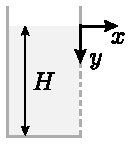
\includegraphics[width=\linewidth]{2015-lahg-07-veejoadJoon}%
\end{wrapfigure}
Small holes at numerous different heights have been made into the wall of a vertical cylindrical vessel and water is flowing out of them. Additional water is slowly poured into the vessel so that the water level inside the vessel is constantly at a height $H$. Find what region of room can the exiting water reach, in other words express the equation for the envelope of the water spurts in $xy$-coordinates. Assume that different water spurts do not affect each other.

\hinteng
To determine what room region the water reaches you can observe the point with coordinates $(x, y)$ and try to determine the initial height of the water spurt for it to reach that point. If there is no solution then the water does not reach such point of room.

\solueng
Let us observe a water spurt that exits the vessel at a location $y=h$. The height of the water column above it is $h$ and from the conservation of energy we can express the initial speed of the exiting spurt: $v=\sqrt{2gh}$. A freely falling water spurt is a parabola, moreover we can describe the movement of one particle with the equations $x=vt$ and $y=h+gt^2/2$. After expressing the time from the first equation we get a parabola’s equation from the second one: $y = h + \frac{gx^2}{2v^2} = h + \frac{x^2}{4h}$. Let us now try to figure out how to determine the room region which the falling water spurts can reach. We could choose a room point $(x,y)$ and ask from what initial height $h$ can this point be reached. To find the suitable initial height $h$ we should solve a quadratic equation $h^2 - yh + x^2/4 = 0$. If the discriminant of this equation is positive then two different solutions can be found for $h$ and the point $(x,y)$ can be reached from two different initial heights. IF the discriminant is negative there are no real-valued solutions and the point $(x,y)$ cannot be reached. A line separates these two cases where the discriminant is zero, meaning $y^2 - x^2=0$, from this we can express the line, meaning the equation for the envelope of the water spurts: $y=x$.
\probend